%!TEX encoding = UTF-8 Unicode
\documentclass[12pt]{article} 
\usepackage[left=0.75in,top=20mm,right=0.75in,bottom=0.3in]{geometry} % Document margins
\usepackage{CJK}
\usepackage{graphicx}
\usepackage{mathtools}
\usepackage{mathrsfs}
\usepackage{amssymb}
\usepackage{hyperref}
\usepackage{sidecap}
\usepackage{makecell}
\usepackage{fancyhdr}
\usepackage{hhline}

\fancypagestyle{title}{
  \setlength{\headheight}{15pt}
  \fancyhf{}
  \renewcommand{\headrulewidth}{0pt}
  \renewcommand{\footrulewidth}{0pt}
  \fancyhead[R]{Parallel Programming 2015}
}

\pagestyle{title}

\makeatletter
\renewenvironment{itemize}
{\list{$\bullet$}{\leftmargin\z@ \labelwidth\z@ \itemindent-\leftmargin
\let\makelabel\descriptionlabel}}
{\endlist}
\makeatother

\begin{CJK}{UTF8}{bsmi}
\title{\textbf{ Homework 4 / Blocked All-Pairs Shortest Path }}
\author{\textbf{李豪韋 (HW-Lee) ID 103061527}}
\date{}

\begin{document}
\vspace*{-60pt}
{\let\newpage\relax\maketitle}
\thispagestyle{title}

\section*{Overview}
\vspace{-20pt}
\noindent\makebox[\linewidth]{\rule{\textwidth}{0.4pt}}
\vspace{5pt}

Given a directed graph, where each pair of vertices has two edges of two directions, APSP (All-pairs shortest path) describes a procedure that obtains all shortest path between each pair of vertices iteratively. The main idea of each iteration is
\begin{center}
    $\text{dist}(i \to j) = \min\big\{ \text{dist}(i \to j), \,\, \text{dist}(i \to k) + \text{dist}(k \to j) \big\} \,\, \forall k \in \mathbb{V}$
\end{center}
which means the distance will be updated by determining whether the vertex $k$ should be passed by when the vertex $i$ is travelling to the vertex $j$. After updating all $k$ at all pairs of vertices, the results must be the shortest path. However, this algorithm does not consider any path with loops, e.g. $v_2 \to v_4 \to v_2 \to v_3$, and we must be sure that loops can only increase the distance. Therefore, it works based on a condition: there is no negative loop within the graph, i.e. the sum of weights of a loop is non-negative.

The algorithm can be parallelized and implemented to be computed by GPU with blocked-APSP, which requires the same computational complexity but less dependency at each iteration. Just like metrices multiplication, the list is separated into several small blocks, and the list can be regarded as a much smaller list which consists of blocks. In this way, it brings some issues: 1) The iteration time $k$ is decreased but the computation of each iteration is more complicated, 2) The situation where the number of vertices is not divisible by determined block size should be well-handled.

\begin{center}
    \begin{figure}[ht]
        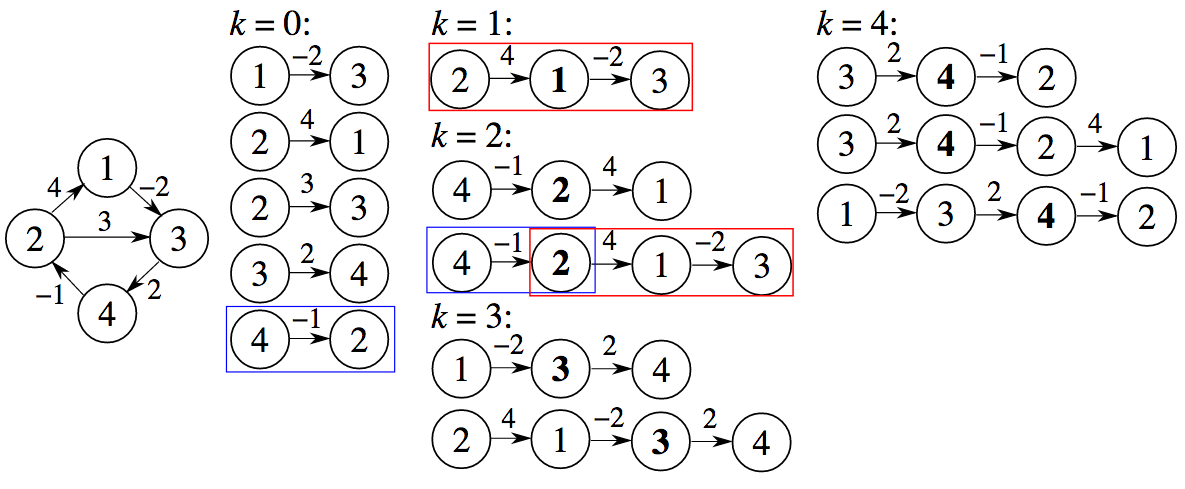
\includegraphics[scale=.45]{./Floyd-Warshall_example.png}
        \caption{A toy example of Floyd-Warshall algorithm (from WIKI)}
    \end{figure}
\end{center}

\newpage

\section*{Implementation}
\vspace{-20pt}
\noindent\makebox[\linewidth]{\rule{\textwidth}{0.4pt}}

\begin{itemize}
    \item Blocks
    \begin{flushleft}
        Supposed that there are $N$ vertices, and the list will be divided into $K^2$ blocks, where each block is $bs$-length. To solve the non-divisible cases, $N$ will be 'padded' at the begining, says $N_{ext}$, then the relation can be derived: $N_{ext} = N + (bs - \mod(N, bs))$, $N_{ext} = K \times bs$. For convenience to index values on the list, there are four indexing variables used in the algorithm: ($b_i$, $b_j$) and ($i$, $j$) denote blocks and pairs relatively. For instance, $B(3, 7)(0, 0)$ refers to the left-upper value of the block coloured with brown in the figure shown below. Therefore, the relation between $D(d_i, \,\, d_j)$ and $B(b_i, \,\, b_j)(i, \,\, j)$ is
        $
        \begin{cases}
            d_i = bs \times b_i + i \\
            d_j = bs \times b_j + j
        \end{cases}
        $
    \end{flushleft}
    \begin{figure}[ht]
        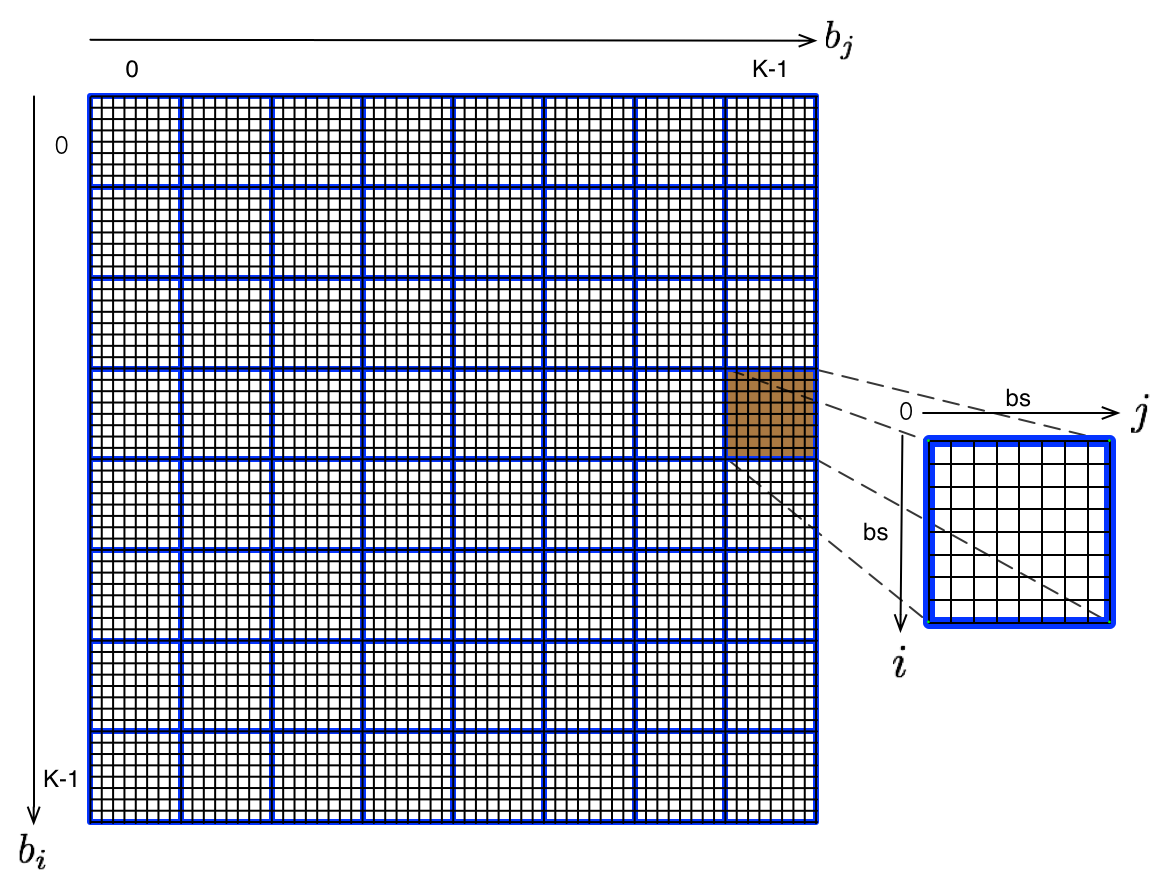
\includegraphics[scale=.4]{./block_indexing.png}
        \caption{Block indexing}
    \end{figure}

    \newpage
    \item Pseudo code
    \vspace{-10pt}
    \begin{align*}
        &\mathsf{function \,\, Update} \,\, B(b_i, \,\, b_j) \,\, \mathsf{do} \makebox[.5\textwidth]{} \\  
        &\quad \quad \mathsf{for } \,\, \mathit{k} = 0:bs-1 \\
        &\quad \quad \quad \quad \mathsf{for } \,\, \mathit{(i, j)} \, \in \, [0, \,\, bs-1]^2 \\
        &\quad \quad \quad \quad \quad \quad B(b_i, \,\, b_j)(i, \,\, j) = \min\big\{B(b_i, \,\, b_j)(i, \,\, j), \,\, B(b_i, \,\, r)(i, \,\, k) + B(r, \,\, b_j)(k, \,\, j)\big\} \\
        &\quad \quad \quad \quad \mathsf{endfor} \\
        &\quad \quad \mathsf{endfor} \\
        &\mathsf{endfunction} \\ \\
        &\mathsf{function \,\, blockFW \,\, do} \\
        &\quad \quad D_{GPU} \leftarrow D_{CPU} \\
        &\quad \quad \mathsf{for} \,\, \mathit{r} = 0:K-1  \\
        &\quad \quad \quad \quad \mathsf{Sync} \big( D_{GPU}, \,\, D_{CPU} \big) \\
        &\quad \quad \quad \quad \mathsf{Update} \,\, B(r, \,\, r) \\
        &\quad \quad \quad \quad \mathsf{Update} \,\, B(r, \,\, 0:K-1) \\
        &\quad \quad \quad \quad \mathsf{Update} \,\, B(0:K-1, \,\, r) \\
        &\quad \quad \quad \quad \mathsf{Update} \,\, B(0:K-1, \,\, 0:K-1) \\
        &\quad \quad \quad \quad \mathsf{Sync} \big( D_{CPU}, \,\, D_{GPU} \big) \\
        &\quad \quad \mathsf{endfor} \\
        &\quad \quad D_{CPU} \leftarrow D_{GPU} \\
        &\mathsf{endfunction}
    \end{align*}
    \vspace{-10pt}
    \begin{SCfigure}[][ht]
        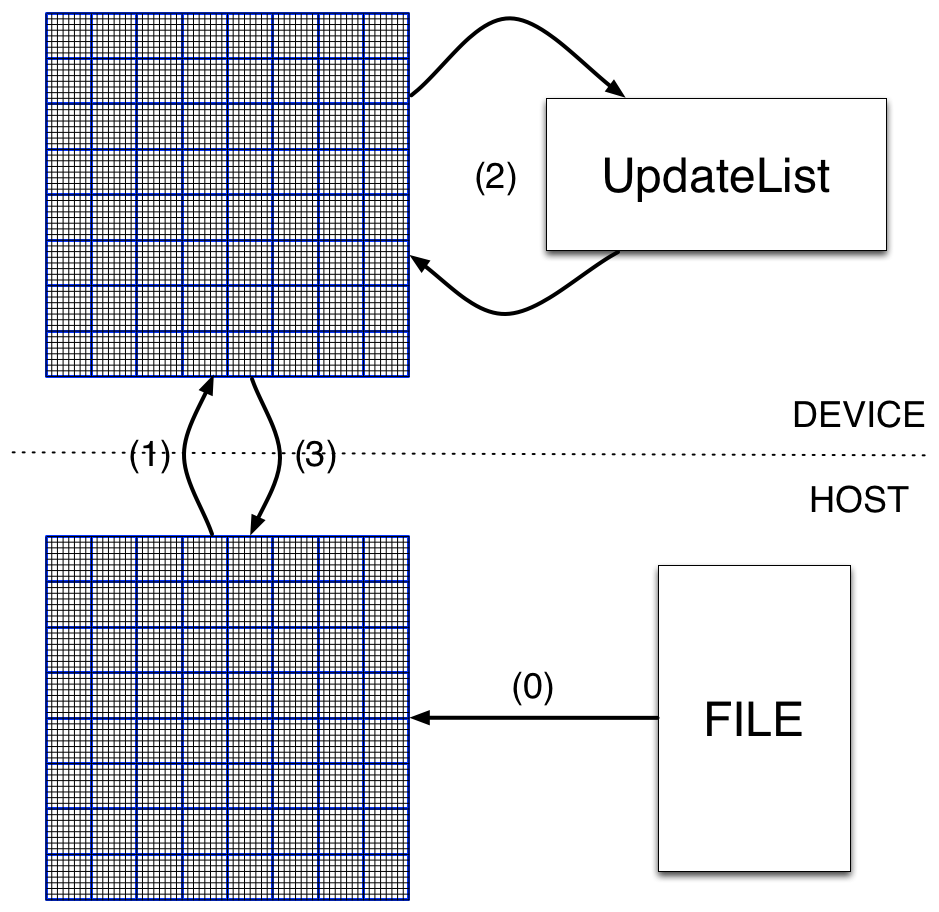
\includegraphics[scale=.3]{./algo_diagram.png}
        \caption{The diagram of the algorithm: the file is loaded first, then send to GPU and update, finally send back to CPU. The operation will be repeated $K$ times}
    \end{SCfigure}

    \newpage
    \item Shared memory in a multiprocessor
    \begin{flushleft}
        In GPU, the shared memory is almost as fast as registers, it offers efficiency when the data needed to be loaded/written are stored in shared memory. For some synchronization issues, a good strategy is to make each multiprocessor owns/processes a block. In addition, according to the updating rules:
        \begin{center}
            $B(b_i, \,\, b_j)(i, \,\, j) = \min\big\{B(b_i, \,\, b_j)(i, \,\, j), \,\, B(b_i, \,\, r)(i, \,\, k) + B(r, \,\, b_j)(k, \,\, j)\big\}$
        \end{center}
        There are only three blocks used to update the list.
        As a result, I assign the shared memory in each multiprocessor to store three blocks, namely $B(b_i, \,\, b_j)$, $B(b_i, \,\, r)$, and $B(r, \,\, b_j)$. In this way, each block can be updated simultaneously and there is no communication with global memory during updating operation. After finishing the operation, the block will be stored back to global memory. This strategy reduces the communication between  multiprocessors and global memory such that the memory bandwidth can be always high enough to transfer data. After all, the operations in a multiprocessor are:
        \begin{enumerate}
            \item Move the data to shared memory
            \item Update block
            \item Move back the data to global memory
        \end{enumerate}
    \end{flushleft}
    \begin{figure}[ht]
        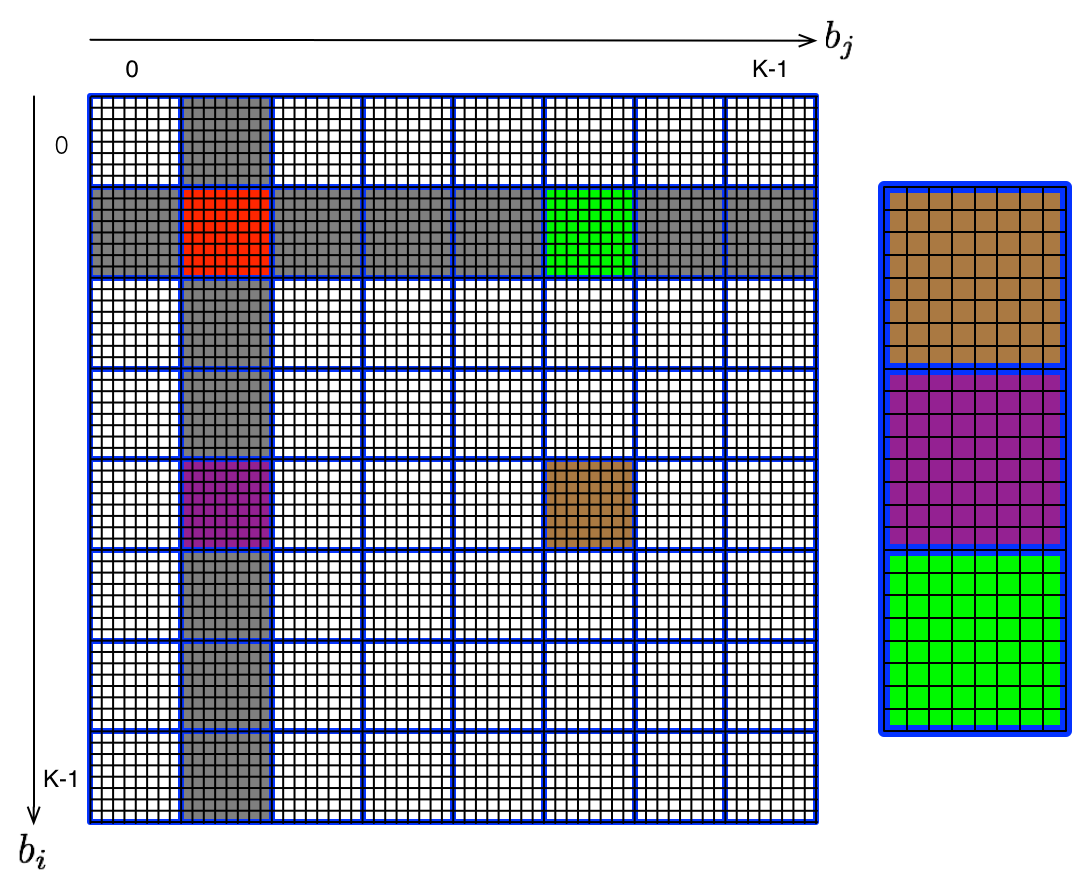
\includegraphics[scale=.4]{./algo_per_block.png}
        \caption{Blocks stored in shared memory per multiprocessor}
    \end{figure}

    \newpage
    \item Multi-GPU
    \begin{flushleft}
        Although GPU has very powerful computation power in parallel programming, it works not fully physically parallel. In GPU architecture, the instructions are executed warp-by-warp, where each warp has several threads, and the number of concurrent warps is limited. Therefore, a kernel task will be executed in serialized ways, it is called logically parallel. However, the performance will be bounded by this physical limitation, we cannot improve it in single GPU. Fortunately, the task still can be done by multi-GPUs with some parallel libraries on CPU like OpenMP and MPI to drive multiple GPUs simultaneously. With multiple GPUs, the physical limitation can be solved but other issues are comming:
        \begin{enumerate}
            \item How to partition the task?
            \item How to synchronize the results?
        \end{enumerate}
        The implementation has been well-tuned so far, and the detail of my optimization progress will be described in the following section. In this section, I only mention the latest implementation. The figure shown below illustrates the instruction at each iteration, the list is divided into two parts, where one GPU processes the upper and another one processes the lower. At the begining of an iteration, CPU copys a row of blocks to GPUs, for guaranteeing that the needed data in the iteration are all correct, which is coloured with yellow. Then all GPUs update the parts of the list they take responsibility for, which are coloured in cyan and green respectively. Finally, CPU should update the data needed in the next iteration from appropriate GPU by copying back the next row of blocks to CPU. After all iteration completed, the task is done. In this way, the communication between each iteration only at the row of the round index, and I/O stage. Consequently, the performance can be improved as two times (even more) as single GPU implementation.
    \end{flushleft}
    \begin{figure}[ht]
        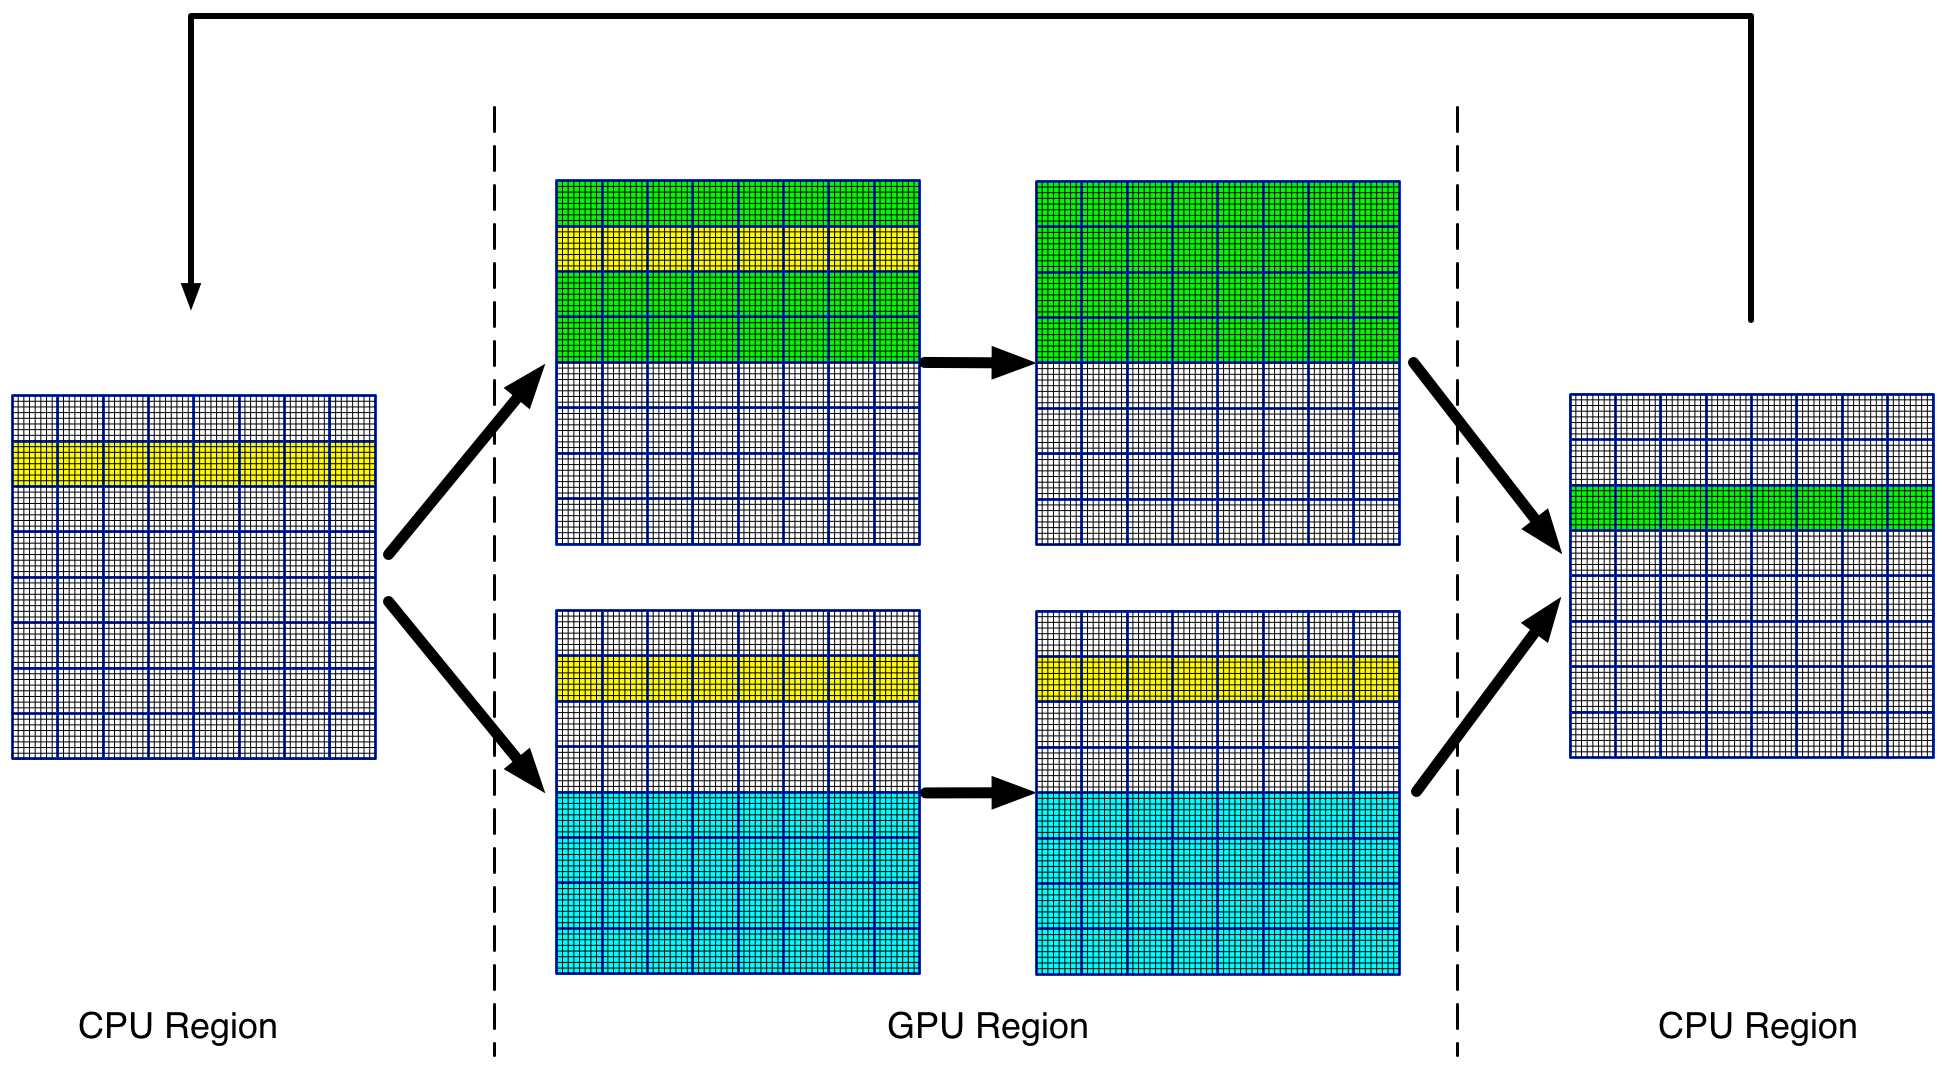
\includegraphics[scale=.25]{./multiGPU_algo_diagram3.png}
        \caption{Multi-GPU implementation diagram at each iteration}
    \end{figure}
\end{itemize}


\section*{Results \& Analysis}
\vspace{-20pt}
\noindent\makebox[\linewidth]{\rule{\textwidth}{0.4pt}}

\begin{itemize}
    \item Weak scalibility (blocking factor is 32, Tesla K20m)
    \begin{flushleft}
        The execution time can be 2-folded with 2 GPUs, the performance is saturated at large number of vertices. The reason why the performance is low at small number of vertices is because the computation is not enough that the time of memory copy really affects the performance.
    \end{flushleft}
    \begin{figure}[ht]
        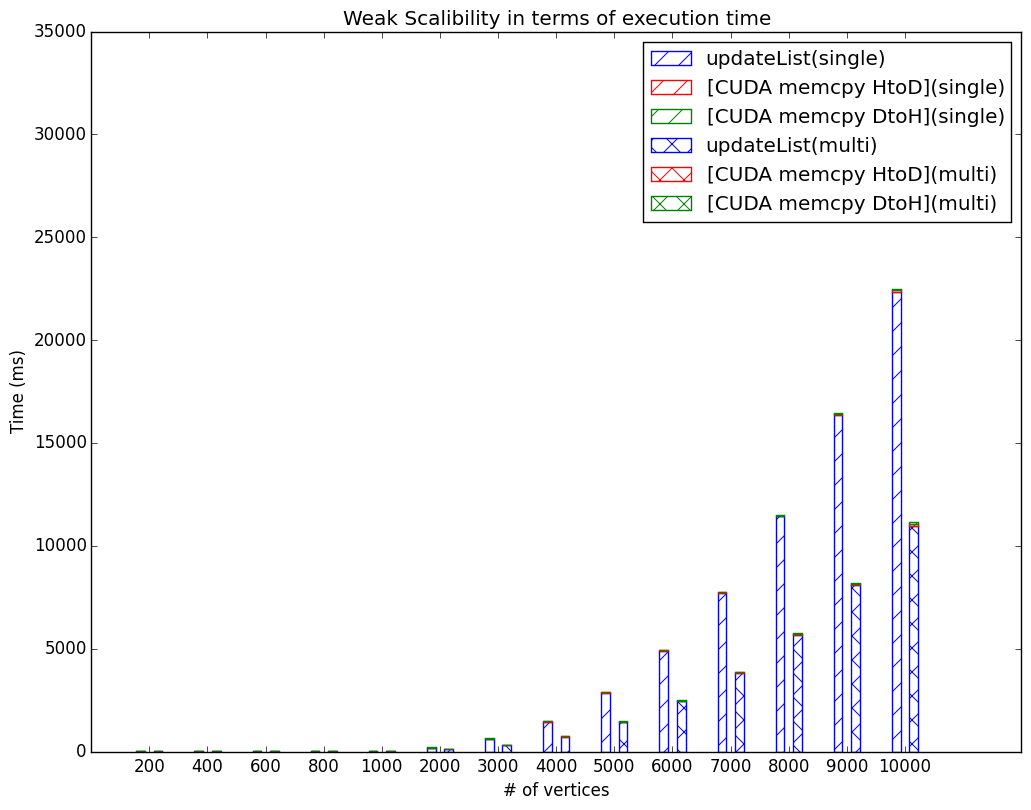
\includegraphics[scale=.5]{./weak-scalibility-time.png}
    \end{figure}
    \begin{figure}[ht]
        \vspace{-20pt}
        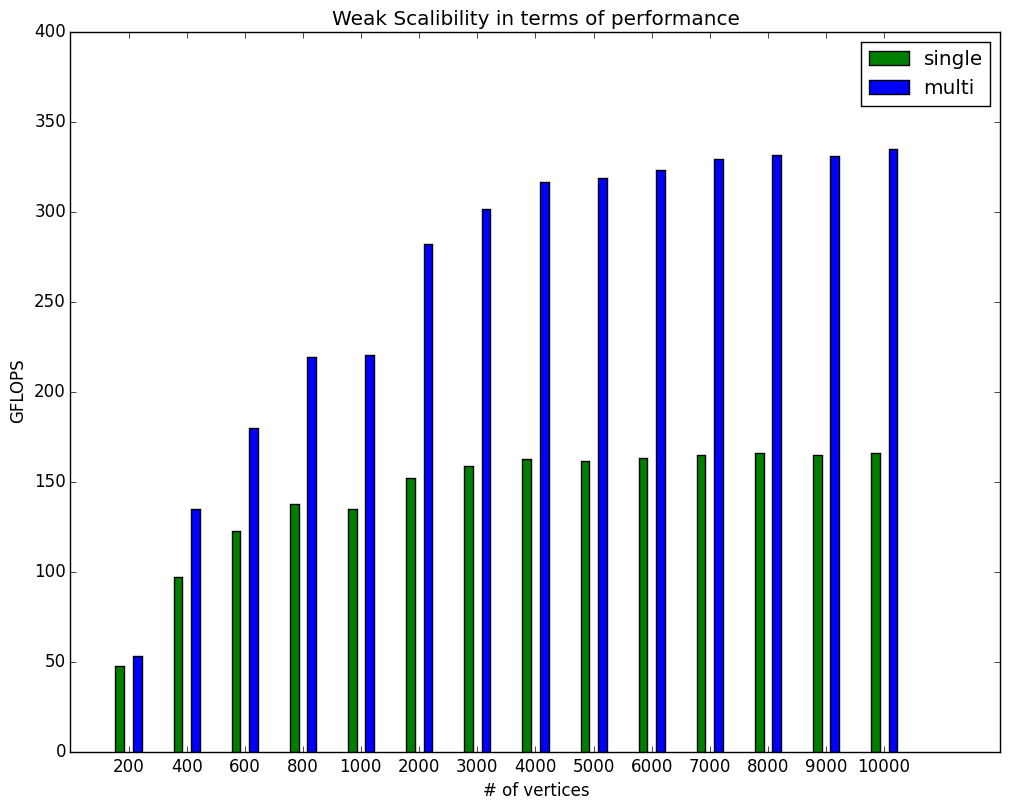
\includegraphics[scale=.5]{./weak-scalibility-perf.png}
        \vspace{-60pt}
    \end{figure}

    \newpage
    \item Blocking factor (6000 vertices, Tesla K20m)
    \begin{flushleft}
        In general, the more factor is used, the less execution time is required. However, the performance decreases when blocking factor changes from 16 to 32, the reason might be caused by the warp size of GPUs. Lower blocking factors induce bad performance because the times copying memory from CPU to GPU and the times doing iteration are more than higher blocking factors, it suffers from kernal launch, memory copy, and synchronization more significantly.
    \end{flushleft}
    \begin{figure}[ht]
        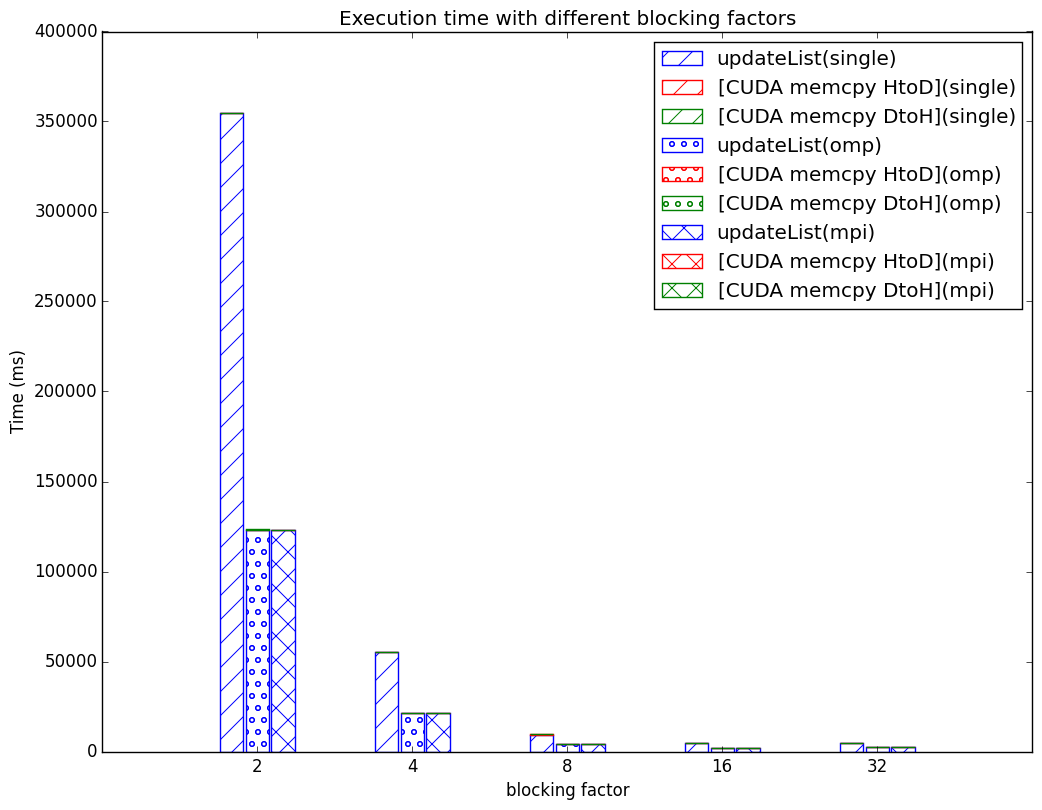
\includegraphics[scale=.5]{./blocking-factor-time.png}
    \end{figure}
    \begin{figure}[ht]
        \vspace{-20pt}
        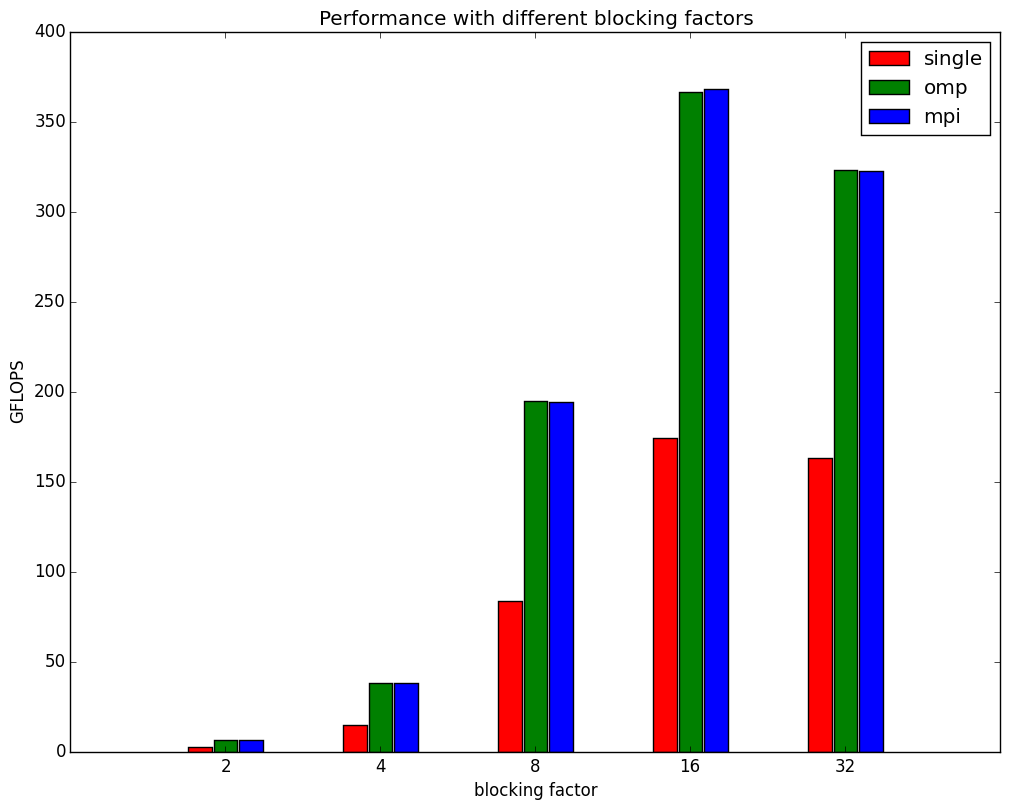
\includegraphics[scale=.5]{./blocking-factor-perf.png}
        \vspace{-60pt}
    \end{figure}

    \newpage
    \item Memory bandwidth in multi-GPU (6000 vertices, Tesla K20m + Tesla K20m)
    \begin{flushleft}
        Lower blocking factors bring lower memory bandwidth, it is because the copy size is so small that constant overhead contributes relatively high time consumption and we cannot ignore this overhead. When the overhead cannot be ignored, it induces larger time consumption and then causes lower memory bandwidth.
    \end{flushleft}
    \begin{figure}[ht]
        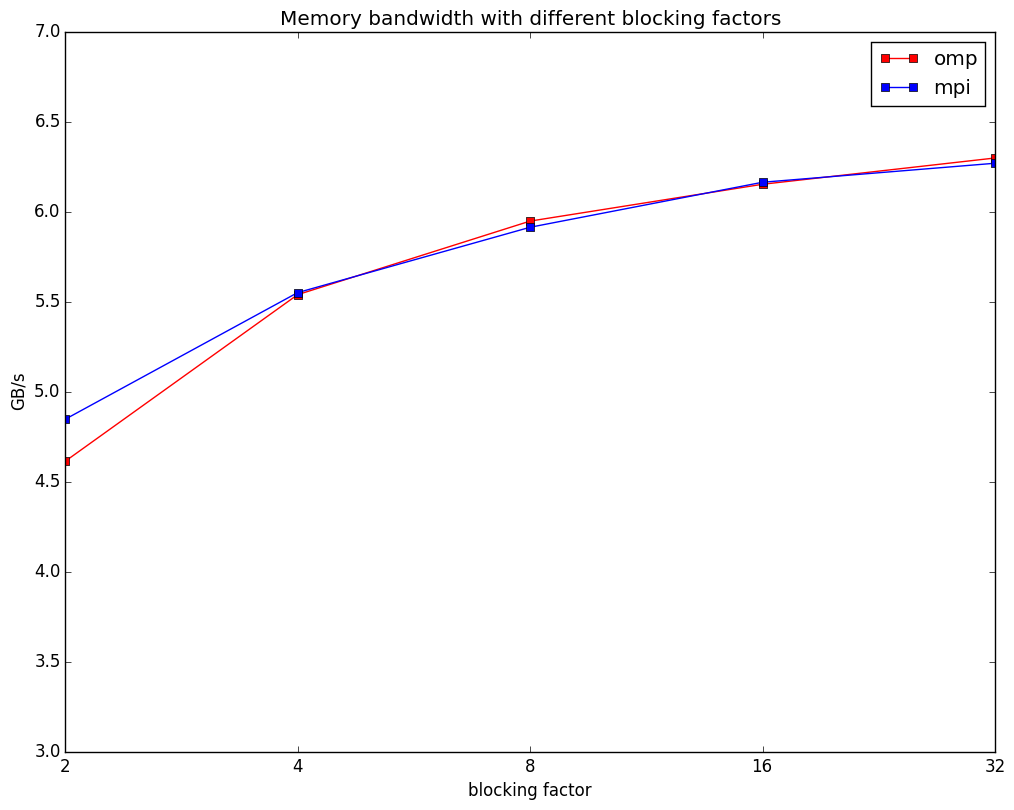
\includegraphics[scale=.5]{./mem-bw.png}
    \end{figure}

    \item Computation time in different phases (6000 vertices, Tesla K20m + Tesla K20m)
    \begin{flushleft}
        The elapsed time in phase 1 will suffer from kernel launch overhead with small block size, because it requires more iterations and then such overhead will be pronounced. According to the difference between time ratio and sequential ratio, there is roughly 1000x faster when using GPUs. It makes sense because GPU can drive hundreds of computation simultaneously.
    \end{flushleft}
    \begin{center}
    \begin{tabular}{|c|c|c|c|c|c|c|c|c|c|}
        \hline
        Configuration & \multicolumn{3}{c|}{$bs = 2$, $K = 3000$} & \multicolumn{3}{c|}{$bs = 4$, $K = 1500$} & \multicolumn{3}{c|}{$bs = 8$, $K = 750$} \\
        \hline
        Phase & 1 & 2 & 3 & 1 & 2 & 3 & 1 & 2 & 3 \\
        \hline
        Elapsed (ms) & 82.96 & 304.82 & 123067.89 & 45.00 & 107.85 & 21096.13 & 21.58 & 42.73 & 4058.65 \\
        \hline
        Time ratio & 1 & 3.674 & 1483.46 & 1 & 2.397 & 468.80 & 1 & 1.98 & 188.07 \\
        \hline
        Seq. ratio & 1 & 6000 & 9000000 & 1 & 3000 & 2250000 & 1 & 1500 & 562500 \\
        \hhline{|==========|}
        Configuration & \multicolumn{3}{c|}{$bs = 16$, $K = 375$} & \multicolumn{3}{c|}{$bs = 32$, $K = 188$} & \multicolumn{3}{c|}{} \\
        \hline
        Phase & 1 & 2 & 3 & 1 & 2 & 3 & & & \\
        \hline
        Elapsed (ms) & 14.90 & 37.40 & 2105.94 & 7.92 & 58.93 & 2376.13 & & & \\
        \hline
        Time ratio & 1 & 2.51 & 141.34 & 1 & 7.44 & 300.02 & & & \\
        \hline
        Seq. ratio & 1 & 750 & 140625 & 1 & 376 & 35344 & & & \\
        \hline
    \end{tabular}
    \end{center}
\end{itemize}

\newpage

\vspace{-10pt}
\section*{Discussion}
\vspace{-20pt}
\noindent\makebox[\linewidth]{\rule{\textwidth}{0.4pt}}

\begin{itemize}
    \item Blocked v.s. normal APSP
    \begin{flushleft}
        There is no difference in terms of complexity between blocked/non-blocked APSP, and the pseudo code of APSP:
        \begin{align*}
            &\mathsf{for} \,\, k = 1:N \,\, \mathsf{do} \\
            &\quad \quad \mathsf{parallel} \,\, \mathsf{foreach} \,\, i, \,\, j \in (1:N)^2 \,\, \mathsf{do} \\
            &\quad \quad \quad \quad d[i][j] = \min\big\{ d[i][j], \,\, d[i][k] + d[k][j] \big\} \\
            &\quad \quad \mathsf{endfor} \\
            &\quad \quad \mathsf{==barrier==} \\
            &\mathsf{endfor}
        \end{align*}
        The instruction can be easily parallelized with shared memory systems like OpenMP and Pthread, and it requires one synchronization step per iteration. However, the advantage is hold only when all threads can see the latest update of the list immediately, i.e. shared memory, it suffers from scalibility issue. In distributed memory systems, the pseudo code is forced to do data synchronization:
        \begin{align*}
            &\mathsf{for} \,\, k = 1:N \,\, \mathsf{do} \\
            &\quad \quad \mathsf{==partition\text{-}data==} \\
            &\quad \quad \mathsf{parallel} \,\, \mathsf{foreach} \,\, i, \,\, j \in (1:N)^2 \,\, \mathsf{do\text{-}local} \\
            &\quad \quad \quad \quad d[i][j] = \min\big\{ d[i][j], \,\, d[i][k] + d[k][j] \big\} \\
            &\quad \quad \mathsf{endfor} \\
            &\quad \quad \mathsf{==merge\text{-}data==} \\
            &\quad \quad \mathsf{==barrier==} \\
            &\mathsf{endfor}
        \end{align*}
        Obviously, it requires more consumption doing data synchronization, and the synchronization cost grows linearly as $k$ increases. To reduce synchronization cost, decreasing iterations is essential for improving performance. As a result, blocked-APSP is used, and the pseudo code has little change: 
        \begin{align*}
            &\mathsf{for} \,\, k = 1:N/bs \,\, \mathsf{do} \\
            &\quad \quad \mathsf{==partition\text{-}data==} \\
            &\quad \quad \mathsf{==phase1\&2\text{-}operation==} \\
            &\quad \quad \mathsf{parallel} \,\, \mathsf{foreach} \,\, b_i, \,\, b_j \in (1:N/bs)^2 \,\, \mathsf{do\text{-}local} \\
            &\quad \quad \quad \quad \mathsf{Update} (B[b_i][b_j]) \\
            &\quad \quad \mathsf{endfor} \\
            &\quad \quad \mathsf{==merge\text{-}data==} \\
            &\quad \quad \mathsf{==barrier==} \\
            &\mathsf{endfor}
        \end{align*}
        In addition to reducing communication, blocked-APSP is chosen for another reason: GPU has shared memory in each multiprocessor, and widely using shared memory can make the performance much better. That's why blocked-APSP is preferred on GPU implementation.
    \end{flushleft}
    \item Single GPU v.s. multiple GPUs
    \begin{flushleft}
        In GPU architecture, there are hundreds of threads residing in a multiprocessor. However, it does not mean that there shall be hundreds of threads running at the same time in a multiprocessor. The compute unit is called stream processor (SM), and each multiprocessor has limited SMs. Because of its limitation, the instructions will be partitioned into several batches which are executed sequentially. It stronly implies that the efficiency of speedup is bounded when the problem size is very large. To enhance its computational speed, using multiple GPUs is proposed. Just like multiple CPUs in past homeworks, using multiple GPUs always requires multiple threads/processes on CPU(s), and the difficulties are more than single GPU implemenation. With multiple GPUs, it increases the computation overlap between threads and reduces some internal costs such as context switch. After all, implementation with multiple GPUs is always superior to that with single GPU.
    \end{flushleft}
    \item Restrictions of the implementation
    \begin{flushleft}
        To optimize the implementation, one of main issues is memory loading/writing. In my implementation, a multiprocessor will store all needed data into its shared memory in advance, and the result shows it does improve the performance very much. However, it brings a limitation: block size. In Tesla K20, the capacity of the shared memory per multiprocessor is only 48KB, and each multiprocessor must store three blocks at each iteration. Therefore, the choice of block size has a small maximal bound: 64 ($64 \times 64 \times 3 \times 4 = 48K$). Fortunately, because of physical limitation, there are only 1024 threads in a multiprocessor, which means the largest blocking factor I can use is only 32, and it is impossible to choose a blocking factor that exceeds 64.
    \end{flushleft}
    \item Blocking factor 16 v.s. 32
    \begin{flushleft}
        In my results, an interesting fact is that the best performance occurs at blocking factor 16 rathor than 32. In general, it does not make sense under same functions (code) if all hardware conditions are optimized. As a result, I think the reasons resulting in this fact is related to hardware implementation. In my implementation, threads and blocks (on GPUs) are requested with multi-dimensional data structures like $\mathsf{dim3}$, I found that if we request threads with integer instead of $\mathsf{dim3}$, then the best performance occurs at blocking factor 32. To explain such result, I think it is caused by this difference. It has been known that the GPU executes instructions warp-by-warp, $\mathsf{dim3}$ might somehow make threads well-distributed and more optimized than linear requesting. All in all, it is still unknown because it might be highly related to hardware issues.
    \end{flushleft}
    \item Branches on GPUs
    \begin{flushleft}
        There is no difference in terms of performance between these two equivalent instructions: $\mathsf{if} \,\, \text{cond}: \,\, a = o_1 \,\, else: \,\, a = o_2$ and $a = o_1 \times \text{cond} + o_2 \times (1-\text{cond})$. The fact shows that 1) there is no branch prediction in GPUs, 2) the cost of branches is roughly equal to the cost of other instructions. Although it is generally suggested to use loops/branches as less as possible, the things really affects the performance is the ratio of using branches of all instructions in a thread. As a result, if the branches are relatively less or can be even ignored, it is totally okay to use branches.
    \end{flushleft}
\end{itemize}

\newpage

\section*{Optimization}
\vspace{-20pt}
\noindent\makebox[\linewidth]{\rule{\textwidth}{0.4pt}}
\vspace{5pt}

This section describes how I improved my algorithm with multiple GPUs and illustrats some comparison to prove that the performance is getting better after each modification.

\begin{itemize}
    \item Synchronize data with whole list
    \begin{figure}[ht]
        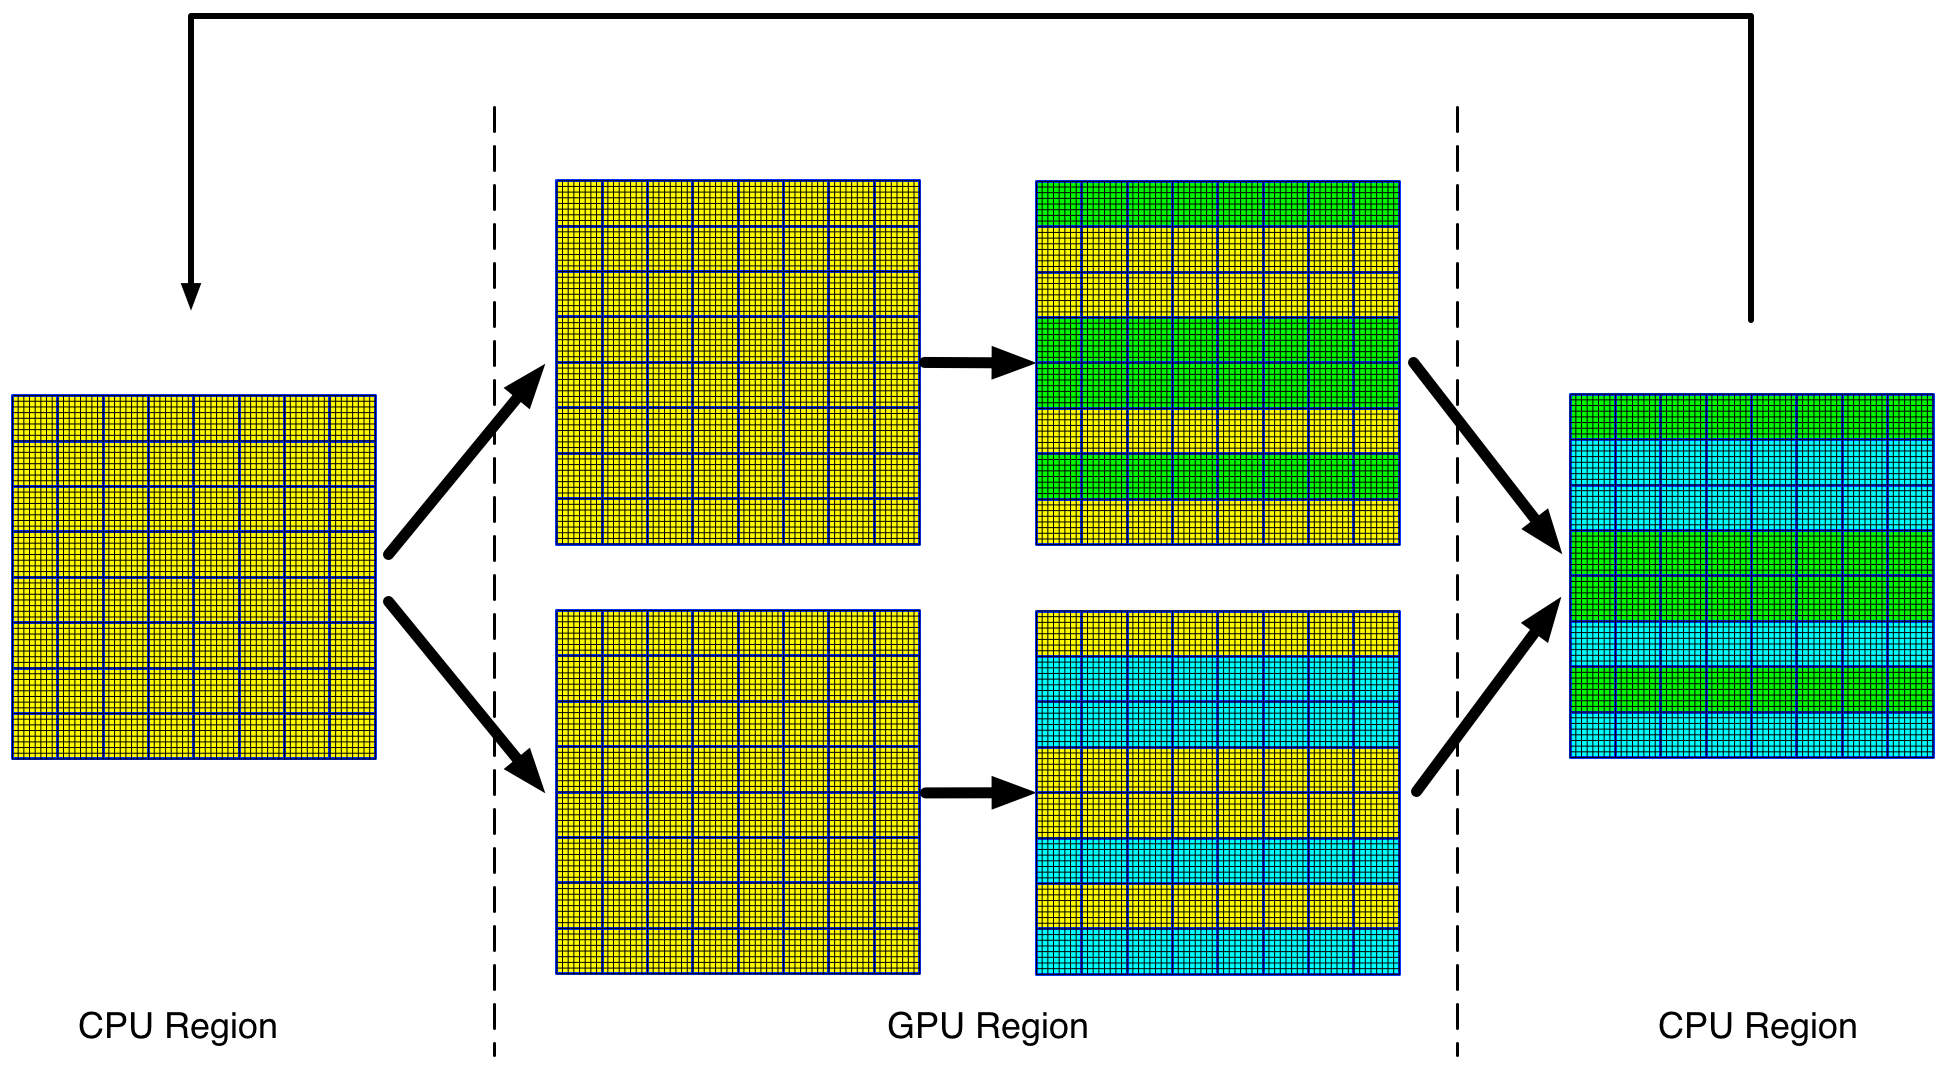
\includegraphics[scale=.25]{./multiGPU_algo_diagram1.png}
        \caption{The first implementation of data synchronization}
    \end{figure}
    \begin{flushleft}
        Expected time ratio between phases should be $1:2(N/bs):(N/bs)^2$, it makes little improvement with parallelizing phase 1 and 2. Therefore, only phase 3 are parallelized with rows. As the figure shown above, the regions in yellow are the data which are transferred from CPU to GPUs at the begining, the regions in yellow/cyan are the data which are assigned to the designated GPUs to compute. In the design, phase 3 computation are partitioned into several rows which are dynamically assigned to multiple GPUs. Because of dynamic scheduling, the updated data must be directly stored back at each iteration.
        \begin{align*}
            &\mathsf{for} \,\, k = 1:N/bs \,\, \mathsf{do} \\
            &\quad \quad \mathsf{MemcpyDtoH} (B[:][:]) \\
            &\quad \quad \mathsf{==phase1\&2\text{-}operation==} \\
            &\quad \quad \mathsf{parallel} \,\, \mathsf{foreach} \,\, b_i = 1:N/bs \,\, \mathsf{do\text{-}local} \\
            &\quad \quad \quad \quad \mathsf{Update} (B[b_i][:]) \\
            &\quad \quad \quad \quad \mathsf{MemcpyDtoH} (B[b_i][:]) \\
            &\quad \quad \mathsf{endfor} \\
            &\quad \quad \mathsf{==barrier==} \\
            &\mathsf{endfor}
        \end{align*}
    \end{flushleft}

    \newpage

    \item Synchronize data with pivot-row and pivot-column
    \begin{figure}[ht]
        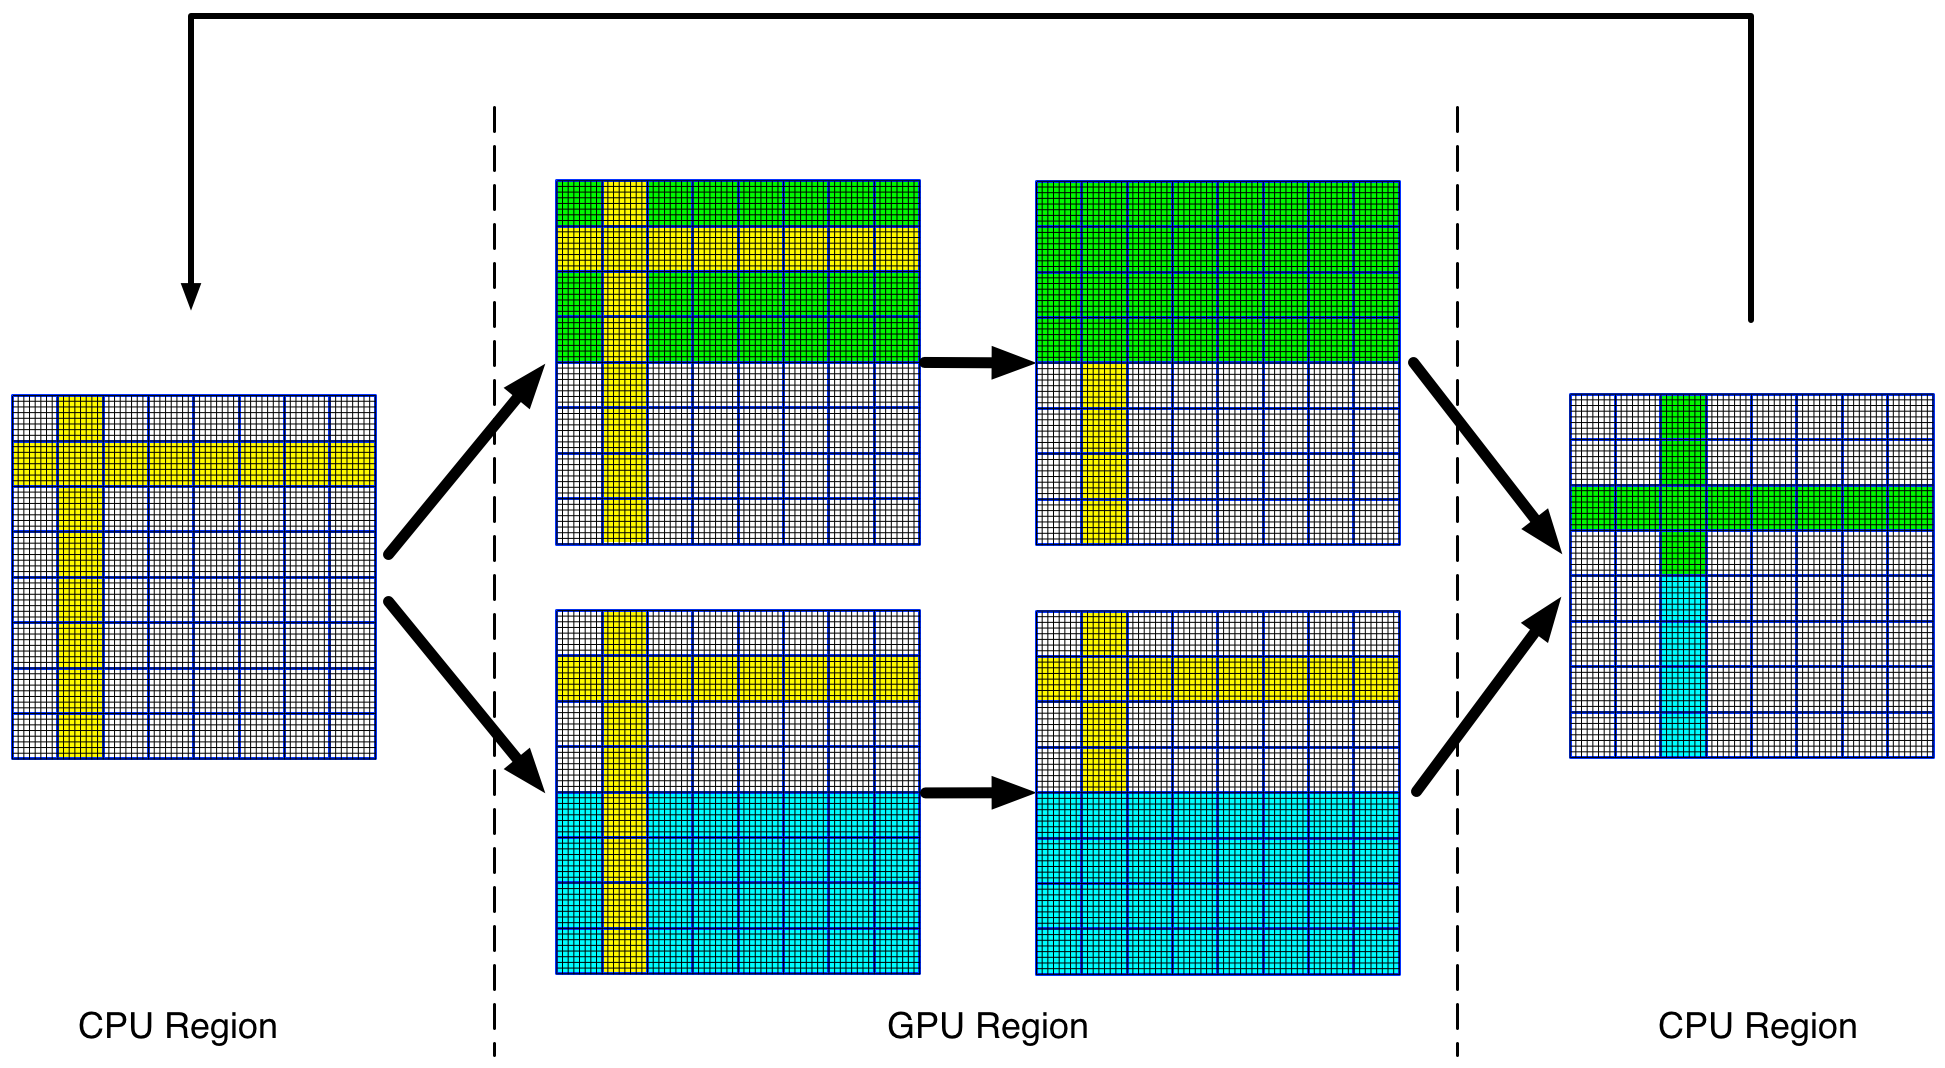
\includegraphics[scale=.25]{./multiGPU_algo_diagram2.png}
        \caption{The second implementation of data synchronization}
    \end{figure}
    \begin{flushleft}
        Because transferring whole list per iteration is a large cost, reducing transferred data is needed. At each iteration, I found that only pivot-row and pivot-column are used, and the other data on GPUs can be reused. However, if only transferring pivot-row and pivot-column, phase 3 computation cannot be dynamically assigned anymore. In this way, it still suffers from one issue: pivot-column communication is a large cost, the way transferring data is to write a loop which does memory copy row by row. The data copied at each row are so small that the required time is dominated by constant latency, and the memory bandwidth is consequently dramatically surppressed, (About 260 MB/s).
        \begin{align*}
            &\mathsf{for} \,\, k = 1:N/bs \,\, \mathsf{do} \\
            &\quad \quad \mathsf{MemcpyDtoH} (B[k][:]) \\
            &\quad \quad \mathsf{MemcpyDtoH} (B[:][k]) \\
            &\quad \quad \mathsf{==phase1\&2\text{-}operation==} \\
            &\quad \quad \mathsf{parallel} \,\, \mathsf{foreach} \,\, b_i = 1:N/bs \,\, \mathsf{do\text{-}local} \\
            &\quad \quad \quad \quad \mathsf{Update} (B[b_i][:]) \\
            &\quad \quad \mathsf{endfor} \\
            &\quad \quad \mathsf{Choose\text{-}Accurate\text{-}MemcpyHtoD} (B[k+1][:]) \\
            &\quad \quad \mathsf{Choose\text{-}Accurate\text{-}MemcpyHtoD} (B[:][k+1]) \\
            &\quad \quad \mathsf{==barrier==} \\
            &\mathsf{endfor}
        \end{align*}
    \end{flushleft}

    \newpage

    \item Synchronize data with pivot-row
    \begin{figure}[ht]
        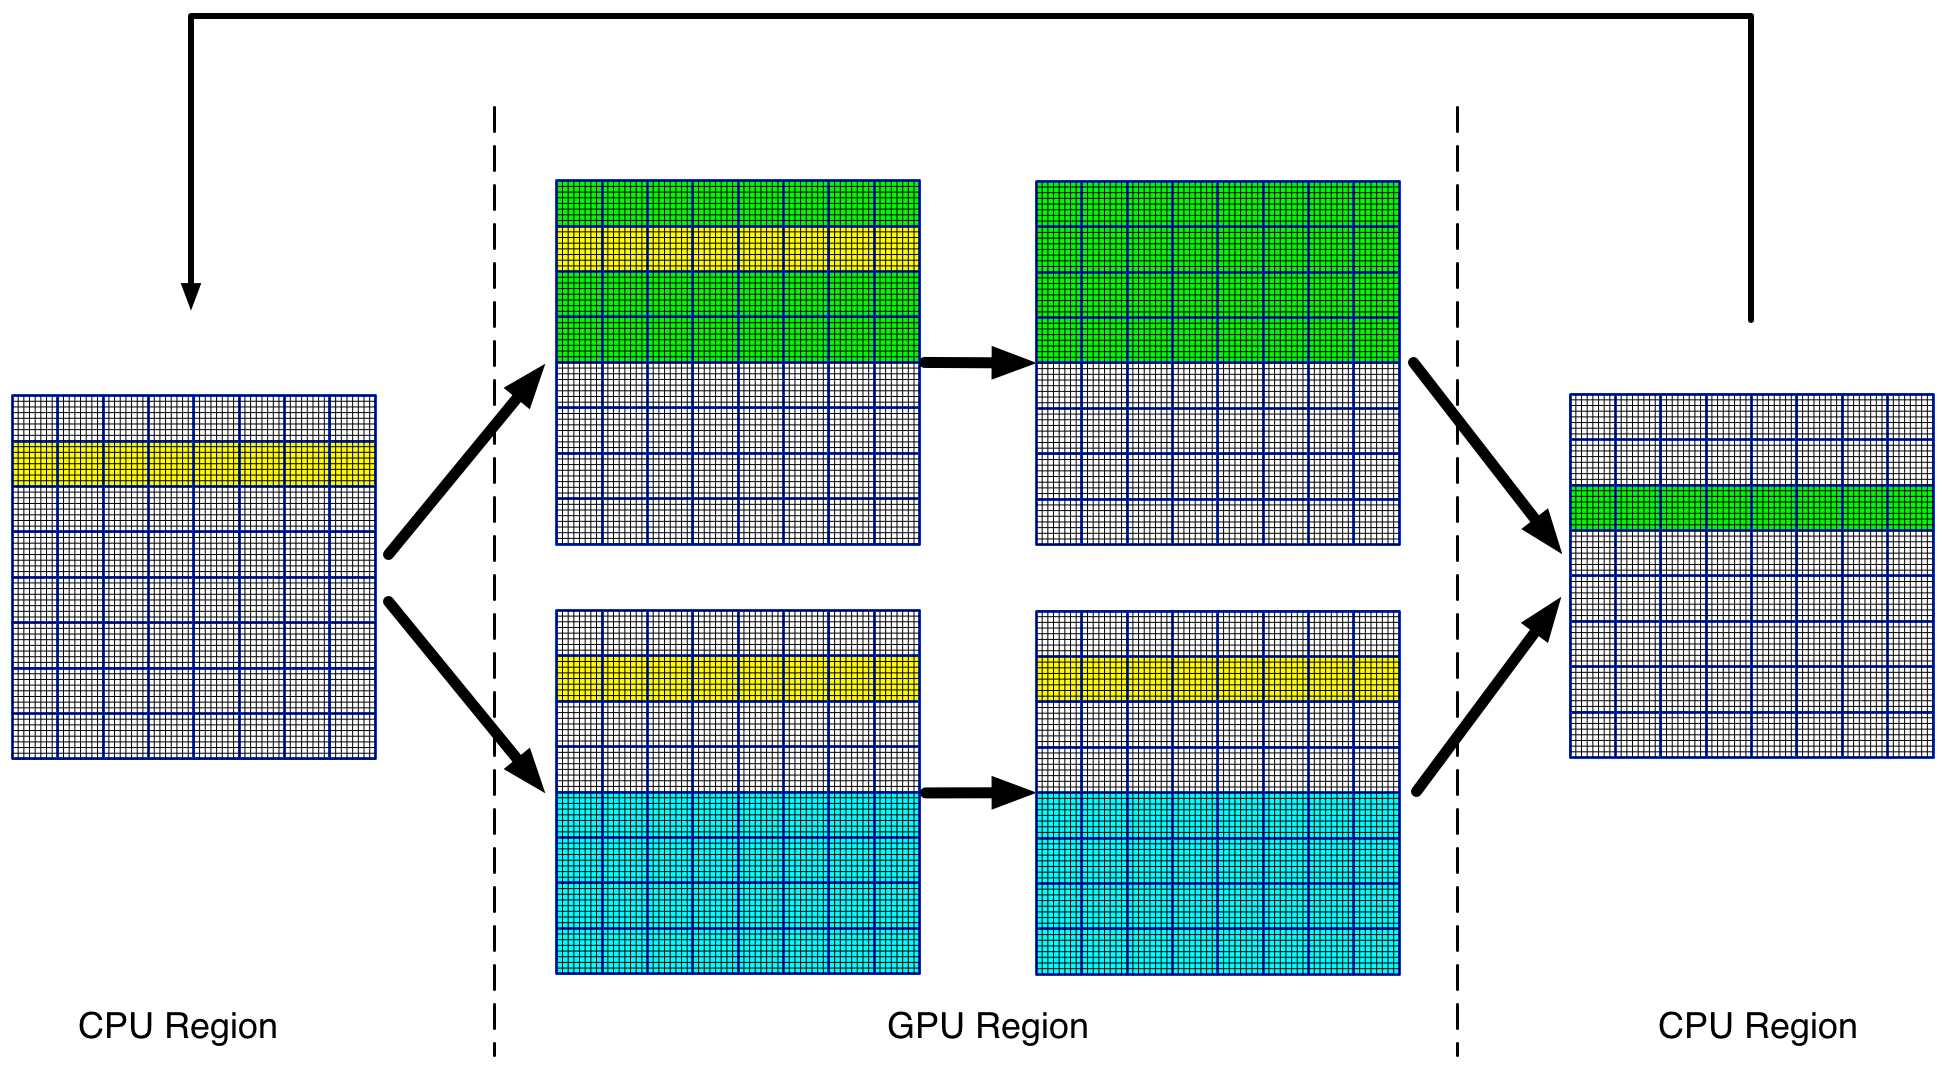
\includegraphics[scale=.25]{./multiGPU_algo_diagram3.png}
        \caption{The third implementation of data synchronization}
    \end{figure}
    \begin{flushleft}
        The time transferring pivot-column is a bottleneck. After analyzing the operation of copying pivot-column, I found that the effect of the operation is only making sure all the pivot-column are the latest values. However, each GPU does not need to make sure the accuracy at blocks it does not need to use. The needed pivot-column has been updated, so the operation is redundant.
        \begin{align*}
            &\mathsf{for} \,\, k = 1:N/bs \,\, \mathsf{do} \\
            &\quad \quad \mathsf{MemcpyDtoH} (B[k][:]) \\
            &\quad \quad \mathsf{==phase1\&2\text{-}operation==} \\
            &\quad \quad \mathsf{parallel} \,\, \mathsf{foreach} \,\, b_i = 1:N/bs \,\, \mathsf{do\text{-}local} \\
            &\quad \quad \quad \quad \mathsf{Update} (B[b_i][:]) \\
            &\quad \quad \mathsf{endfor} \\
            &\quad \quad \mathsf{Choose\text{-}Accurate\text{-}MemcpyHtoD} (B[k+1][:]) \\
            &\quad \quad \mathsf{==barrier==} \\
            &\mathsf{endfor}
        \end{align*}
    \end{flushleft}

    \item Fully unrolled in a thread
    \begin{flushleft}
        As the block size limitation mentioned above, the block size can be greater than 32, which means each thread needs to process more than one value. In practice, loops for making each thread look through all values it should process take lots of time because for-loop is a relatively large cost in GPU implementation. Although the directive description $\mathsf{\# \,\, pragma \,\, unroll}$ is available, the performance is still not improved a lot. Therefore, the final optimization is to re-limit maximal block size to 32 such that each thread only needs to process one value and the for-loops can be removed.
    \end{flushleft}

    \item Overall comparison (blocking factor 64, 6000 vertices)
    \begin{flushleft}
        The overall results between all optimization stages are listed below. According to the table, the largest improvement is to reduce communication cost (see the ratio of Memcpy). The first implementation has high memory bandwidth but requires large data copy, the second implementation reduces data size a lot but suffers from memory bandwidth because of pivot-column copy. Finally, the third and forth implementations are efficient enough and do not suffer from communication, I think it has been optimized and its performance seems to depend mostly on hardware.
    \end{flushleft}
    \begin{center}
    \begin{tabular}{|c|c|c|c|c|c|}
        \hline
        & Memcpy per iteration & Memory bandwidth & updateList & Memcpy HtoD & Memcpy DtoH \\
        \hline
        $1^{st}$ & 144.77MB & 6.06GB/s & 7.02s (51.11\%) & 4.38s (31.90\%) & 2.33s (16.99\%) \\
        \hline
        $2^{nd}$ & 3.0802MB & 3.14GB/s & 6.58s (75.23\%) & 1.14s (13.04\%) & 1.03s (11.73\%)  \\
        \hline
        $3^{rd}$ & 1.5401MB & 6.13GB/s & 6.58s (99.11\%) & 36.6ms (0.55\%) & 22.8ms (0.34\%) \\
        \hline
        $4^{th}$ & 1.5401MB & 6.28GB/s & 2.45s (96.82\%) & 44.5ms (1.76\%) & 35.8ms (1.41\%) \\
        \hline
    \end{tabular}
    \end{center}
\end{itemize}

\end{CJK}
\end{document}